\documentclass[12pt,norsk,a4paper]{article}
\usepackage[norsk]{babel}
\usepackage[norsk]{isodate}
\usepackage[T1]{fontenc}
\usepackage{parskip}
\usepackage{url}
\usepackage{listings}
\author{fridatbe}
\title{IN1080 --- Obligatorisk oppgave 6}
\date{\today}
\usepackage[small,euler-digits]{eulervm}
\usepackage{color}
% \usepackage{minted}
\usepackage{xcolor}
\definecolor{LightGray}{gray}{0.9}
\usepackage{a4wide}
\usepackage[top=2cm]{geometry}
\usepackage{graphicx}
\graphicspath{ {./fig/} }
\newcommand{\tuple}[1]{\ensuremath{\langle #1\rangle}}
\newcommand{\set}[1]{\ensuremath{\{#1\}}}
\newcommand{\imp}{\ensuremath{\rightarrow}}
\newcommand{\M}{\ensuremath{\mathcal{M}}}
\newcommand{\AF}{edge from parent[draw=none]}
\newcommand{\NODE}[1]{\{node \{\ensuremath{#1}\}\}}
\usepackage[explicit]{titlesec}
\titleformat{\section}{\normalfont\Large\bfseries}{}{0em}{#1\ \thesection}


\begin{document}
    \maketitle
    \renewcommand{\thesubsection}{(\alph{subsection})}
    \newpage

    \section{Oppgave}
        Deloppgave A:\\
        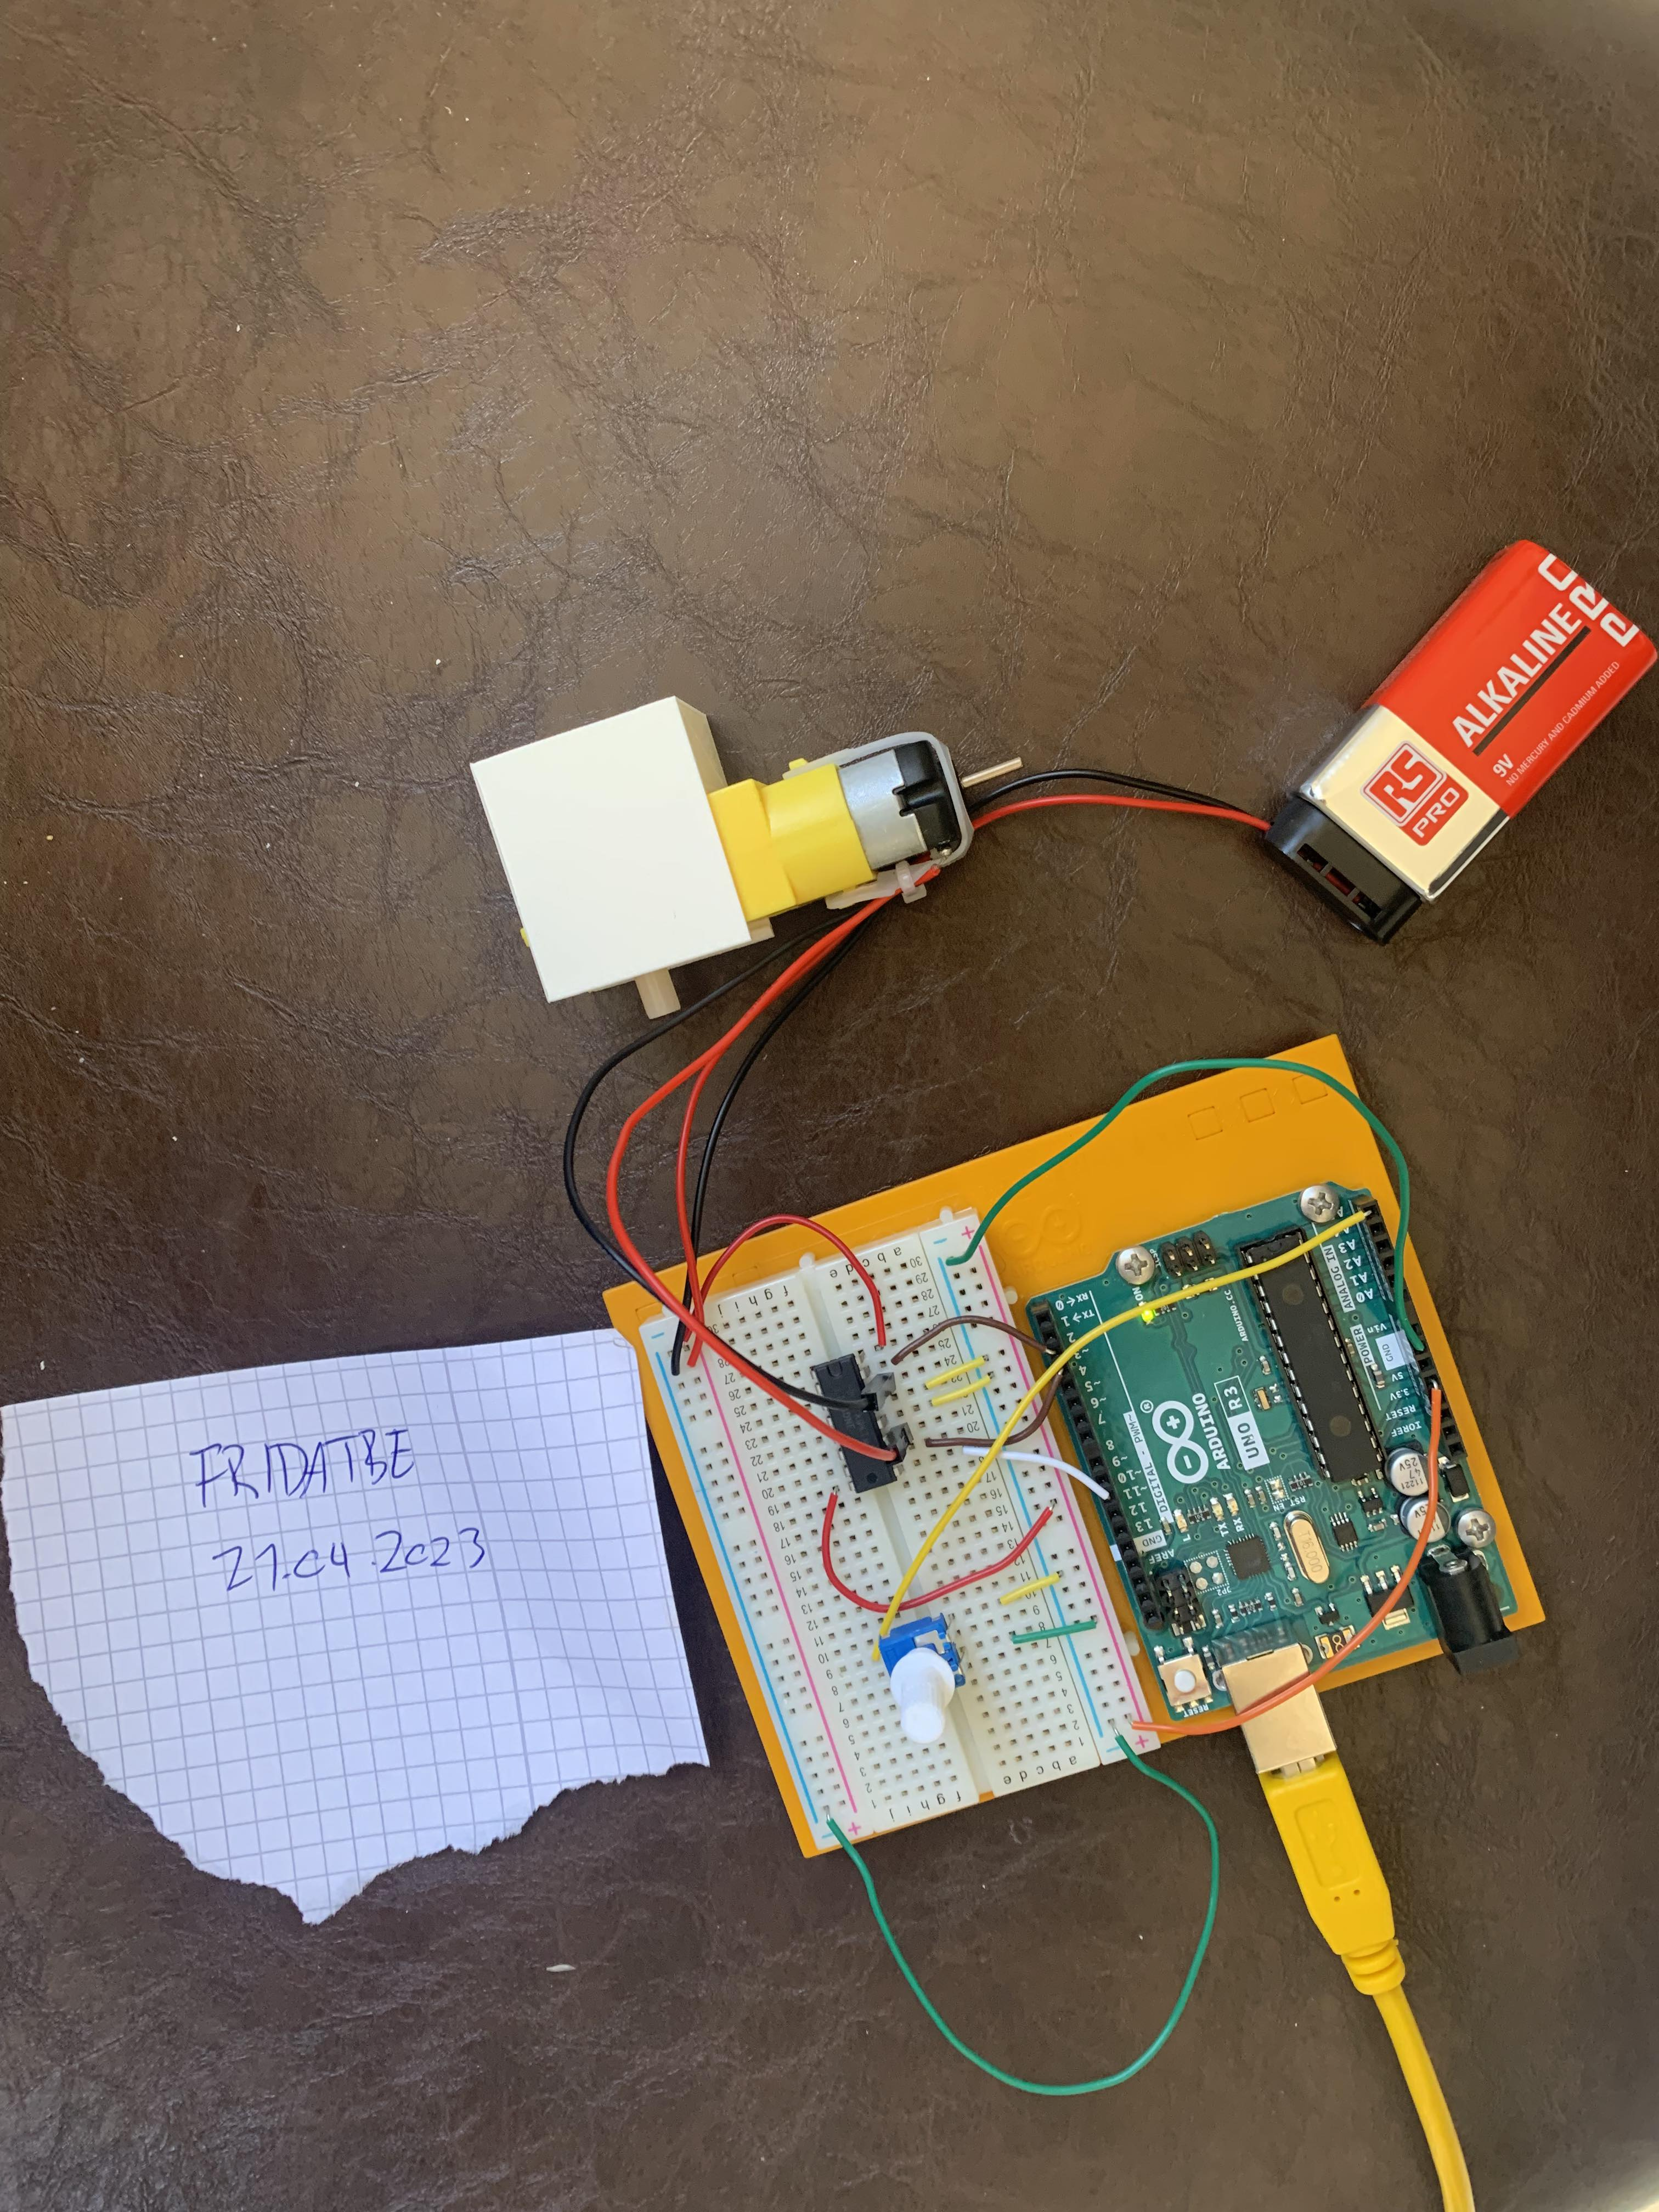
\includegraphics[width=0.5\textwidth]{oppsett.jpg}\\\\

        Deloppgave C:\\
        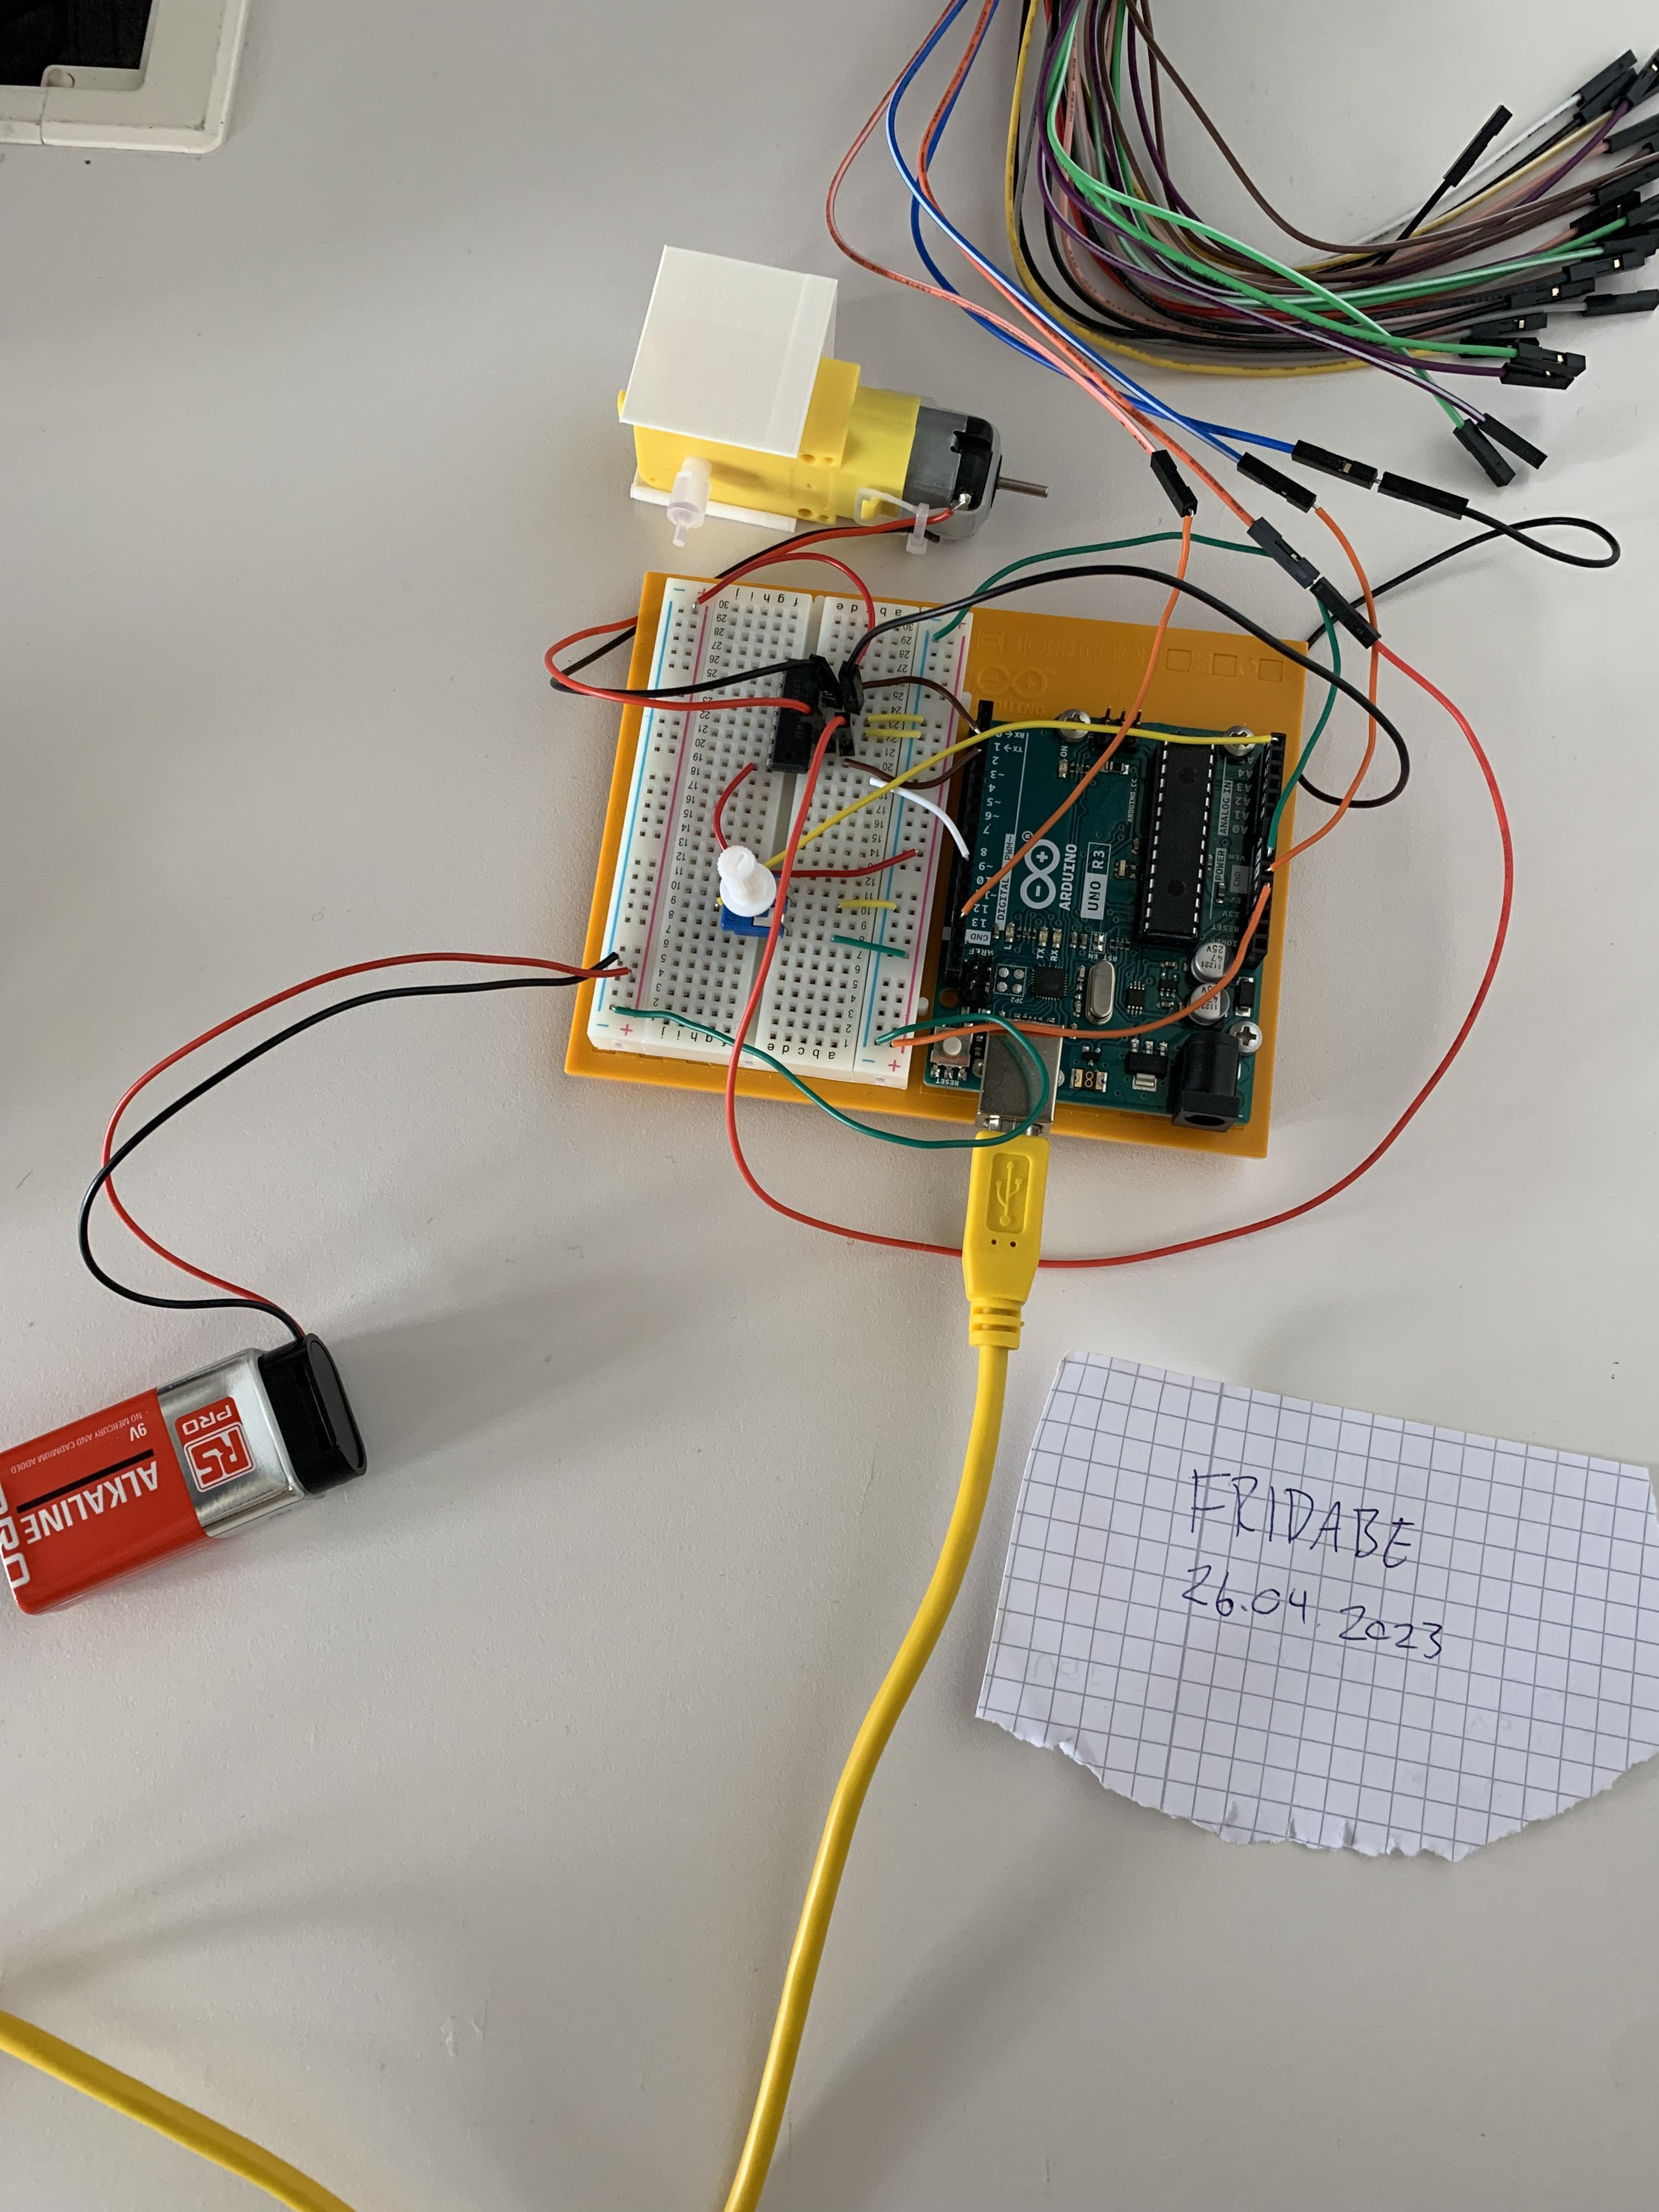
\includegraphics[width=0.5\textwidth]{bilde_oppsett.jpg}\\\\
        Bilde fra scope:\\
        *observerer at signalet ikke oppfører helt som forventet. dette kan nok være fordi selv om enable pin-en er satt til high, er fortsatt pin 2 high. Dette kunne jeg nok ha unngått ved å endre pinMode til low for både pin 2 og 3 der enable også er low i arduino-koden. Men i praksis funket motoren i takt med potentiometeret som forventet\\\\
        
\includegraphics[width=1\textwidth]{screen.png}\\


    \newpage
    \section{Oppgave}
        Det var vanskelig å få endret på PID-konstantene fordi komponentene i kretsen var dårlige. For at motoren skulle rotere måtte jeg presse ned potentiometerene og driveren for at det skulle få kontakt med arduino brødbretett. Så har ikke forslag på P, I og D verdier\\\\
        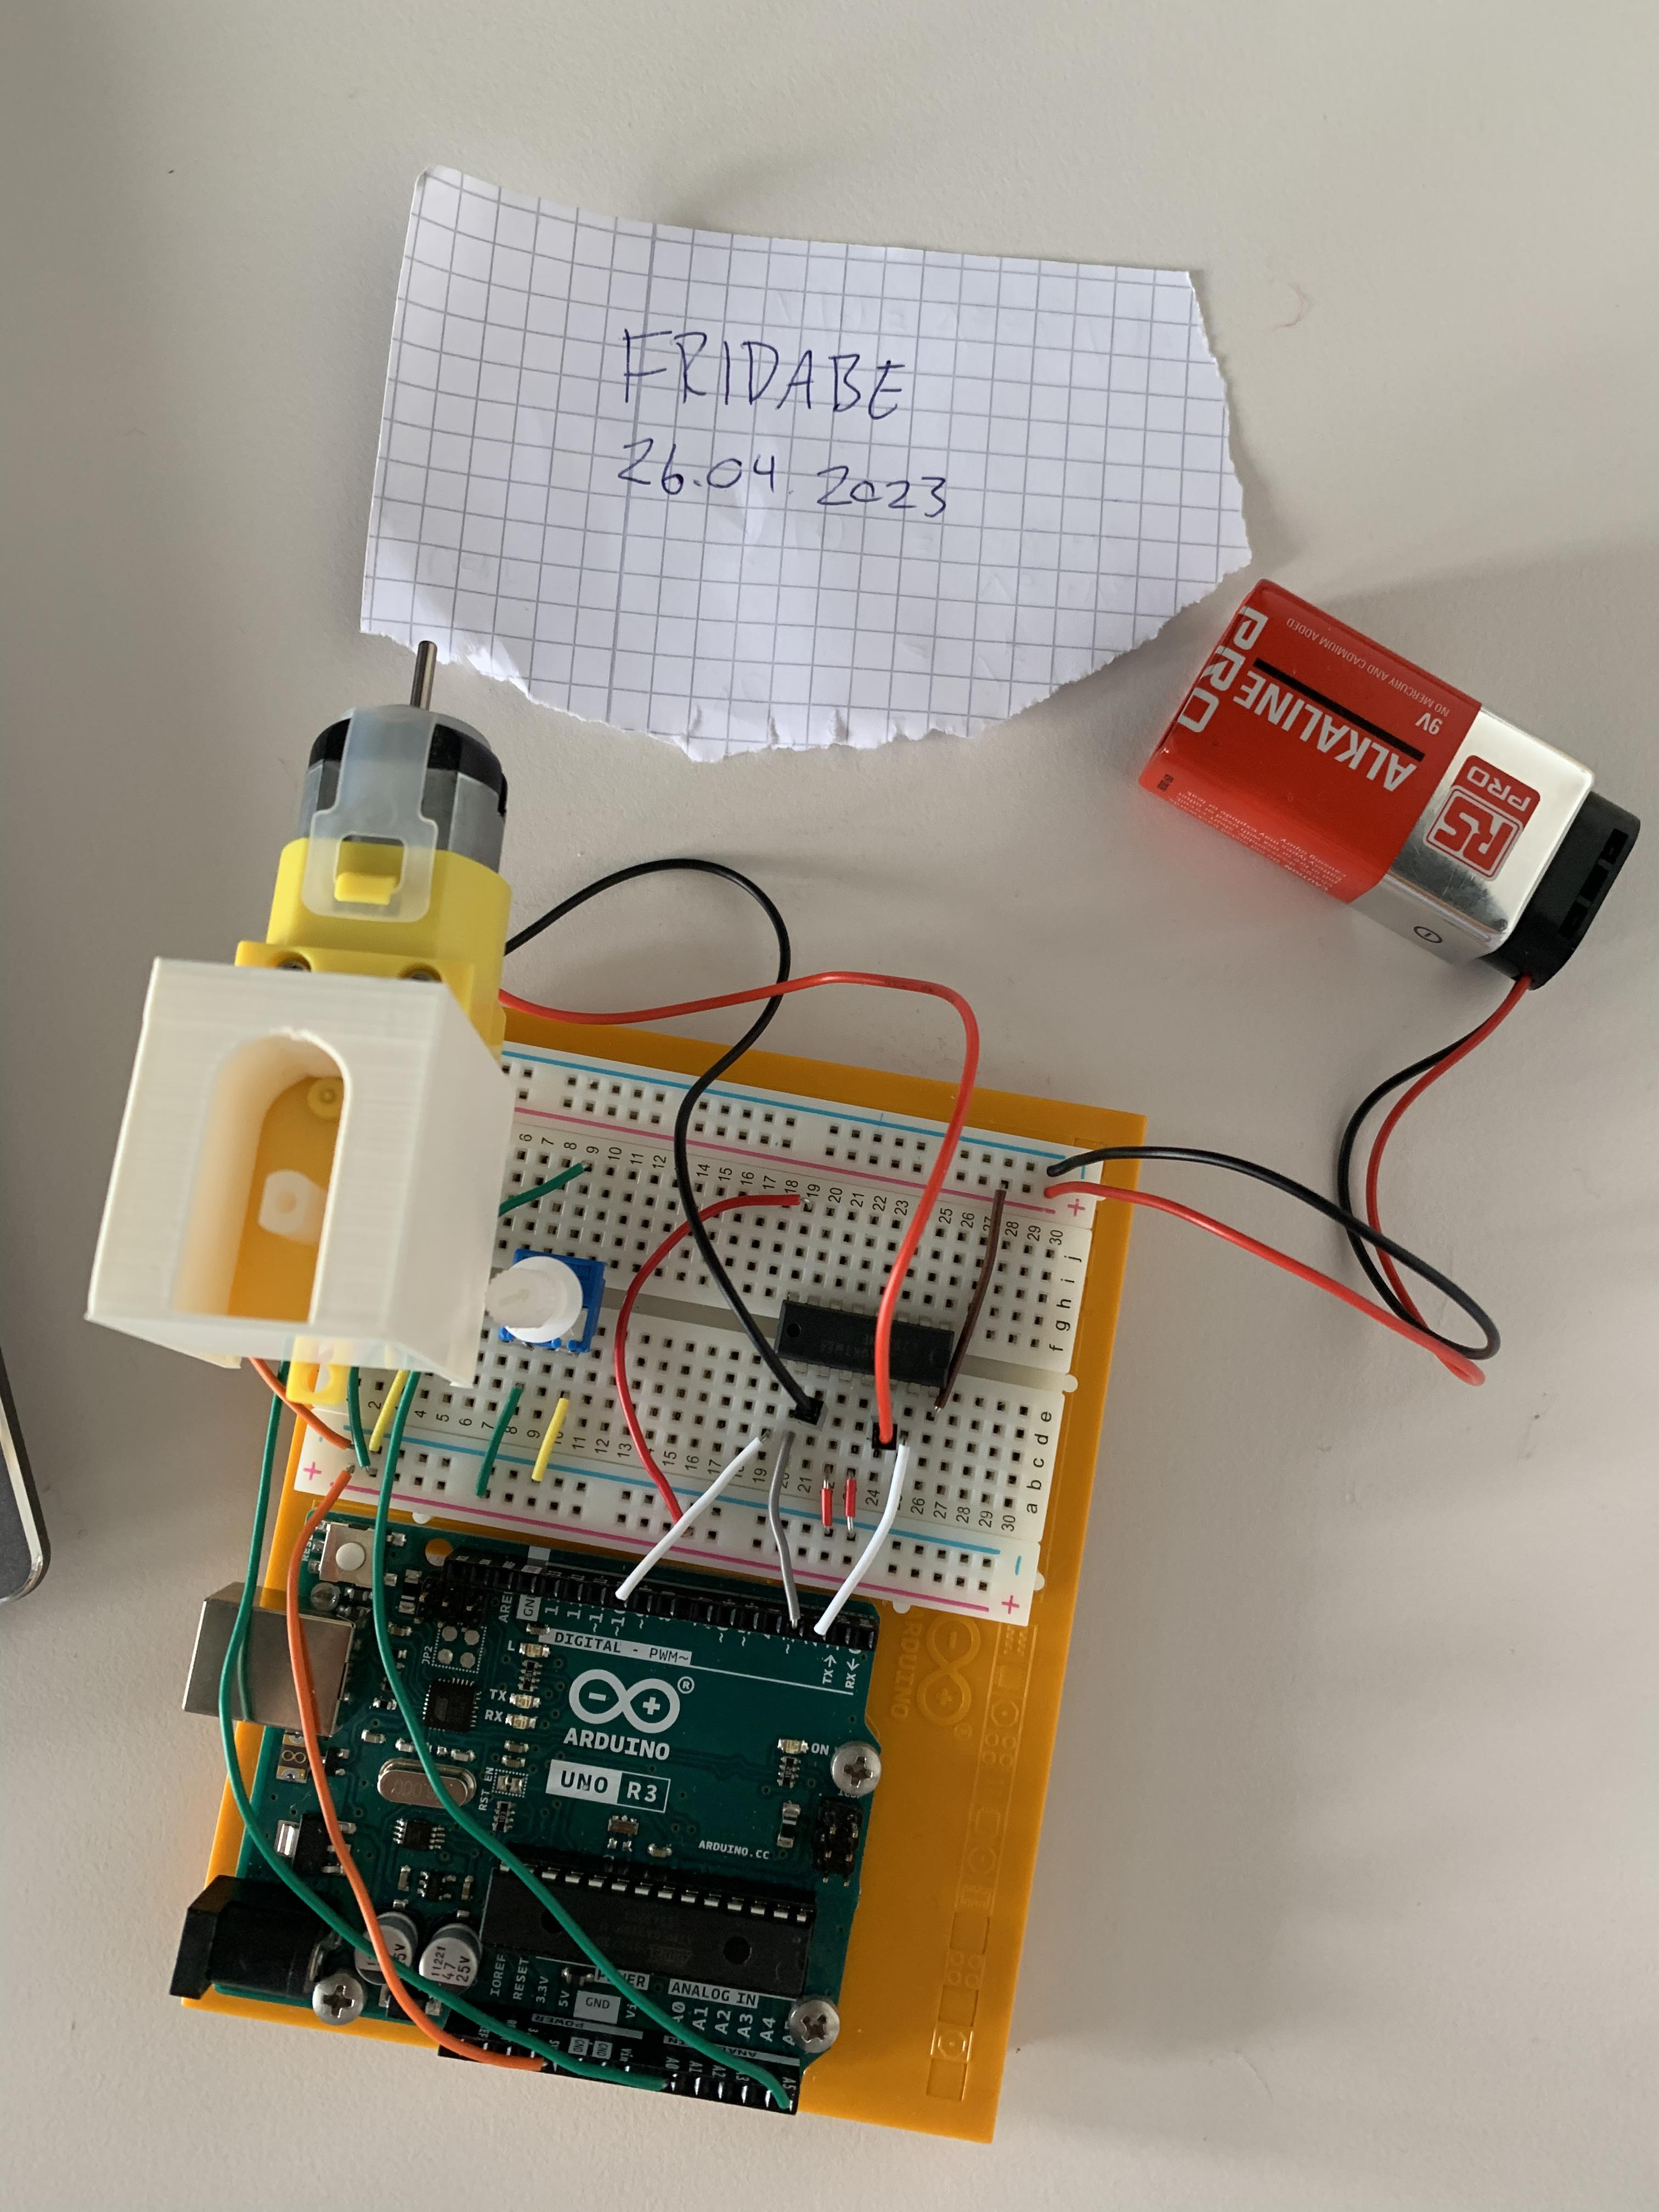
\includegraphics[width=0.7\textwidth]{oppsett2.jpg}\\
    
    
    \newpage

\end{document}
